\def\mytitle{AVR-GCC ASSIGMNMENT}
\def\myauthor{NARENDRA MANIKANTA}
\def\contact{manikantakesana0@gmail.com}
\def\mymodule{Future Wireless Communications (FWC)}
\documentclass[journal,12pt,twocolumn]{IEEEtran}

\usepackage{setspace}
\usepackage{gensymb}
\usepackage{xcolor}
\usepackage{caption}
\usepackage[hyphens,spaces,obeyspaces]{url}
\usepackage[cmex10]{amsmath}
\usepackage{mathtools}
\usepackage{enumitem}
\usepackage{tikz}
\usetikzlibrary{automata, positioning}

\usepackage{enumitem}
\usepackage{circuitikz}
\usepackage{karnaugh-map}
\usepackage{tabularx}
\usepackage{tikz}
\singlespacing
\usepackage{amsthm}
\usepackage{mathrsfs}
\usepackage{txfonts}
\usepackage{stfloats}
\usepackage{cite}
\usepackage{cases}
\usepackage{subfig}
\usepackage{longtable}
\usepackage{multirow}
\twocolumn


\usepackage{graphicx}
\graphicspath{{./images/}}
\usepackage[colorlinks,linkcolor={black},citecolor={blue!80!black},urlcolor={blue!80!black}]{hyperref}
\usepackage[parfill]{parskip}
\usepackage{lmodern}
\usepackage{tikz}
\usepackage{circuitikz}
\usepackage{karnaugh-map}
\usepackage{pgf}
\usepackage[hyphenbreaks]{breakurl}

\usepackage{tabularx}
\usetikzlibrary{calc}

\renewcommand*\familydefault{\sfdefault}
\usepackage{watermark}
\usepackage{lipsum}
\usepackage{xcolor}
\usepackage{listings}
\usepackage{float}
\usepackage{titlesec}
\DeclareMathOperator*{\Res}{Res}
\renewcommand\thesection{\arabic{section}}
\renewcommand\thesubsection{\thesection.\arabic{subsection}}
\renewcommand\thesubsubsection{\thesubsection.\arabic{subsubsection}}

\renewcommand\thesectiondis{\arabic{section}}
\renewcommand\thesubsectiondis{\thesectiondis.\arabic{subsection}}
\renewcommand\thesubsubsectiondis{\thesubsectiondis.\arabic{subsubsection}}
\titlespacing{\subsection}{1pt}{\parskip}{3pt}
\titlespacing{\subsubsection}{0pt}{\parskip}{-\parskip}
\titlespacing{\paragraph}{0pt}{\parskip}{\parskip}
\newcommand{\figuremacro}[5]{
    \begin{figure}[#1]
        \centering
        \includegraphics[width=#5\columnwidth]{#2}
        \caption[#3]{\textbf{#3}#4}
        \label{fig:#2}
    \end{figure}
}

\lstset{
frame=single, 
breaklines=true,
columns=fullflexible
}

%\thiswatermark{\centering \put(400,-128.0){\includegraphics[scale=0.3]{logo}} }
\title{\mytitle}
\author{\myauthor\hspace{1em}\\\contact\\IITH\hspace{0.5em}-\hspace{0.6em}\mymodule}
\date{20-12-2022}
\def\inputGnumericTable{}                                 %%
\lstset{
%language=C,
frame=single, 
breaklines=true,
columns=fullflexible
}
 \begin{document}
%

\theoremstyle{definition}
\newtheorem{theorem}{Theorem}[section]
\newtheorem{problem}{Problem}
\newtheorem{proposition}{Proposition}[section]
\newtheorem{lemma}{Lemma}[section]
\newtheorem{corollary}[theorem]{Corollary}
\newtheorem{example}{Example}[section]
\newtheorem{definition}{Definition}[section]
%\newtheorem{algorithm}{Algorithm}[section]
%\newtheorem{cor}{Corollary}
\newcommand{\BEQA}{\begin{eqnarray}}
\newcommand{\EEQA}{\end{eqnarray}}
\newcommand{\define}{\stackrel{\triangle}{=}}
\bibliographystyle{IEEEtran}

\vspace{3cm}
\maketitle
\tableofcontents
\section{\textbf{Question}}
A Boolean function $F$ of three $X$, $Y$ and $Z$ is given as $F(X,Y,Z)=(X' + Y+ Z)\cdot(X + Y'+ Z')\cdot(X' Y + Z')\cdot(X'Y'Z' + X'YZ' + XYZ')$. Which one of the following is true?
\vspace{1.5mm}
\begin{enumerate}[label=(\alph*)]
    \item $F(X, Y, Z)=(X + Y+ Z')\cdot(X' + Y' + Z')$
    \item $F(X, Y, Z)=(X' + Y)\cdot(X + Y' + Z')$
    \item $F(X, Y, Z)=X'Z' + YZ'$
    \item $F(X, Y, Z)=X'Y'Z + XYZ$
\end{enumerate}
    \section{\textbf{Answer}}
    The above question can reduced as follows \\
    $\rightarrow (X' + Y + Z)\cdot(X' + Y + Z')\cdot(X + Y' +Z')\cdot(X'Y'Z' + X'YZ' + XYZ')$\\
    $\rightarrow(X' + Y)\cdot(X + Y' + Z')\cdot(X'Z' + XYZ')$\\
    $\rightarrow(X' + Y)\cdot(X + Y' + Z')\cdot(X'Z' + YZ')$\\
    $\rightarrow(X'Y' + X'Z' + YX + YZ')\cdot(X'Z' + YZ')$\\
    $\rightarrow X'Y'Z' + X'Z' + X'YZ' + XYZ' + X'YZ' + YZ'$\\
    $\rightarrow X'Z' + YZ' + YZ'$\\
    $\rightarrow X'Z' + YZ'$\\
    Therefore, the Boolean function $F(X, Y, Z)=(X' + Y)\cdot Z'$
   \section{\textbf{Logic Diagram}}
   \begin{center}
       
   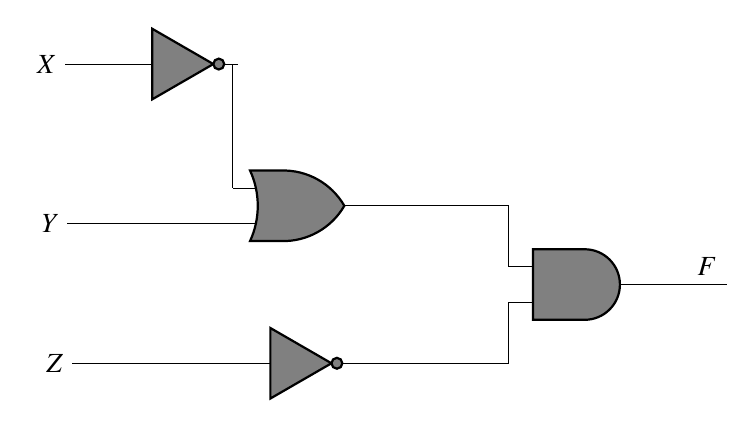
\begin{tikzpicture}
\ctikzset{
    logic ports=ieee,
    logic ports/scale=0.8,
    logic ports/fill=gray
}
 
% Logic ports
\node[not port] (notx) at (1,-0.2){};
\node[or port] (ora) at (2.5,-2){};
\node[not port]  (notz) at (2.5,-4){};
\node[and port] (andf) at (6,-3){};
 \draw(notx.out)-|(ora.in 1);
 \draw(notz.out)-|(andf.in 2);
 \draw(ora.out)-|(andf.in 1);
 \draw(andf.out)-- ++(1.05,0) node[near end,above]{$F$};
 \draw(notz.in)-- ++(-2.2,0) node[left]{$Z$};
 \draw(ora.in 2)-- ++(-2.1,0) node[left]{$Y$};
 \draw(notx.in)-- ++(-0.8,0) node[left]{$X$};


\end{tikzpicture}
\begin{center}
Fig. 1 
\end{center}
       \end{center}







 \section{\textbf{Truth Table}}
\begin{tabularx}{0.45\textwidth}{
  | >{\centering\arraybackslash}X  
  %| >{\centering\arraybackslash}X 
  %| >{\centering\arraybackslash}X
 % | >{\centering\arraybackslash}X 
 % | >{\centering\arraybackslash}X 
  %| >{\centering\arraybackslash}X 
 % | >{\centering\arraybackslash}X 
  | >{\centering\arraybackslash}X 
  | >{\centering\arraybackslash}X 
  | >{\centering\arraybackslash}X |
  }
  \hline
  \textbf{$X$}&\textbf{$Y$}&\textbf{$Z$}&\textbf{$F$}\\
  \hline
  0&0&0&1\\
  \hline
  0&0&1&0\\
  \hline
  0&1&0&1\\
  \hline
  0&1&1&0\\
  \hline
  1&0&0&0\\
  \hline
  1&0&1&0\\
  \hline
  1&1&0&1\\
  \hline
  1&1&1&0\\
  \hline
  
    \end{tabularx}
     \begin{center}
 Truth table for Boolean Function $F$
\end{center}

  \section{\textbf{K-Map Implementation}}
    Using the boolean logic output $F$ can be expressed in terms of the inputs $X,Y,Z$ with the help of the following Kmap.
\\
    \begin{center}
      \resizebox{0.45\textwidth}{!}{%
      \begin{karnaugh-map}[4][2][1][$YZ$][$X$]
            \maxterms{1,4,5,3,7}
            \minterms{0,2,6}
            \implicant{2}{6}
            \implicantedge{0}{0}{2}{2}
        \end{karnaugh-map}%
        }
    \end{center}
    \begin{center}
Fig. 2
\end{center}
\begin{center}
    \section{\textbf{Components}}
  \begin{tabularx}{0.45\textwidth} { 
  | >{\centering\arraybackslash}X 
  | >{\centering\arraybackslash}X 
  | >{\centering\arraybackslash}X
  | >{\centering\arraybackslash}X | }
\hline
 \textbf{Component}& \textbf{Values} & \textbf{Quantity}\\
\hline
Arduino & UNO & 1 \\  
\hline
Jumper Wires& M-M & 5 \\ 
\hline
Breadboard &  & 1 \\
\hline
\end{tabularx}
\end{center}




\begin{center}
    \section{\textbf{Implementation}}
  \begin{tabularx}{0.46\textwidth} { 
  | >{\centering\arraybackslash}X 
  | >{\centering\arraybackslash}X 
  |>{\centering\arraybackslash}X  | }


\hline
\textbf{Arduino PIN} & \textbf{INPUT} & \textbf{OUTPUT} \\ 
\hline
\textbf 5& X & \\
\hline
\textbf 6 & Y & \\
\hline
\textbf 7 & Z & \\
\hline
\textbf 2 & & F \\
\hline
\end{tabularx}
\end{center}
\begin{center}
    Connections
\end{center}

\textbf{Procedure}\\
1. Connect the circuit as per the above table.\\
2. Connect inputs to Vcc for logic 1, ground for logic 0.\\
3. Execute the circuit using the below code.\\
\\\begin{tabularx}{0.45\textwidth} { 
  | >{\centering\arraybackslash}X |
 % | >{\centering\arraybackslash}X |
 }
  \hline
https://github.com/arduinojinarendra/\\fwc\_1may/blob/main/avr\-gcc\_code/main\.c\\
  \hline
\end{tabularx}



\bibliographystyle{ieeetr}
\end{document}


       
       
 \bibliographystyle{ieeetr}
\end{document}
